%This work is licensed under the Creative Commons License Attribution 4.0 International (CC-BY 4.0)
%https://creativecommons.org/licenses/by/4.0/legalcode
\documentclass[rgb]{standalone}
\usepackage{pgfplots}
\definecolor{myorange}{hsb}{0.0833, 1, 0.8}
\definecolor{mygreen}{hsb}{0.3333, 1, 0.8}
\definecolor{myblue}{hsb}{0.5833, 1, 0.8}
\definecolor{mymagenta}{hsb}{0.8333, 1, 0.8}
\begin{document}
	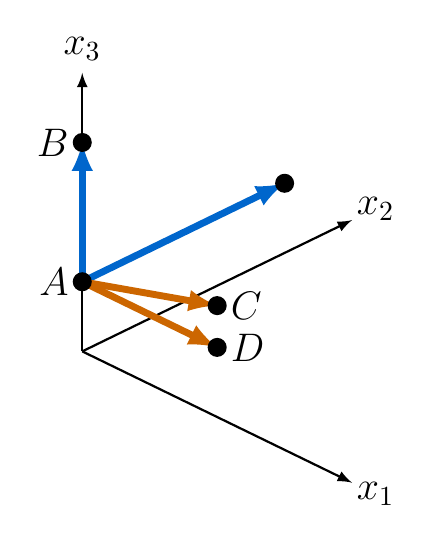
\begin{tikzpicture}[font=\Large]
		\begin{axis}[scale=1.5,clip=false,hide axis,grid=none, minor tick num =1,view={135}{45}, xmin=-3,xmax=3, ymin=-3,ymax=3, zmin=0, zmax=4, ztick={0,2,4}, xlabel=$x_1$, ylabel=$x_2$, zlabel=$x_3$]	
			\draw[thick, -latex] (axis cs:0,0,0) -- (axis cs:0,0,4);
			\draw[thick, -latex] (axis cs:0,0,0) -- (axis cs:0,4,0);
			\draw[thick, -latex] (axis cs:0,0,0) -- (axis cs:-4,0,0);
			\draw[line width=2.5pt, myblue, -latex] (axis cs:0,0,1) -- (axis cs:0,0,3);
			\draw[line width=2.5pt, myblue, -latex] (axis cs:0,0,1) -- (axis cs:-3,0,1);
			\draw[line width=2.5pt, myorange, -latex] (axis cs:0,0,1) -- (axis cs:0,2,1);
			\draw[line width=2.5pt, myorange, -latex] (axis cs:0,0,1) -- (axis cs:0,2,1.6);
			\node at (axis cs:-4.35,0,0) [anchor= center] {$x_2$};	
			\node at (axis cs:0,4.35,0) [anchor= center] {$x_1$};	
			\node at (axis cs:0,0,4.35) [anchor= center] {$x_3$};	
			\node at (axis cs:0,0,1) [left=0.5mm] {$A$};	
			\node at (axis cs:0,0,3) [left=0.5mm] {$B$};	
			\node at (axis cs:0,2,1) [right=0.5mm] {$D$};	
			\node at (axis cs:0,2,1.6) [right=0.5mm] {$C$};	
			\node[very thick, draw, circle,fill,inner sep=2] at (axis cs:0,0,1) {};		
			\node[very thick, draw, circle,fill,inner sep=2] at (axis cs:0,0,3) {};	
			\node[very thick, draw, circle,fill,inner sep=2] at (axis cs:-3,0,1) {};	
			\node[very thick, draw, circle,fill,inner sep=2] at (axis cs:0,2,1) {};	
			\node[very thick, draw, circle,fill,inner sep=2] at (axis cs:0,2,1.6) {};	
		\end{axis}
	\end{tikzpicture}
\end{document}